% id: 111-54
% book: 쎈B 대수 · 08 등차수열과 등비수열
% section: 유형 12 등차수열의 합의 활용
% figure: tikz:fig-111-54
% answer: 
% answer_source: 
% variant_level: 0 (원본 전사)
% 이 파일은 build.mjs 가 items.json 에서 만든다. 고칠 때는 items.json 을 고친다.
\smash{\raisebox{1.5mm}{\dmkichul{쎈B 대수 111쪽 54번}}}
\noindent\begin{minipage}[t]{0.58\linewidth}\vspace{0pt}\raggedright 오른쪽 그림과 같이 직선 $l$ 위에 같은 간격으로 $20$개의 점 $\pt{P_1}$, $\pt{P_2}$, $\pt{P_3}$, $\cdots$, $\pt{P_{20}}$을 잡고, 각 점에서 직선 $m$에 내린 수선의 발을 차례대로 $\pt{Q_1}$, $\pt{Q_2}$, $\pt{Q_3}$, $\cdots$, $\pt{Q_{20}}$이라 하자. $\seg{P_1Q_1}=7$, $\seg{P_{20}Q_{20}}=13$일 때, $\seg{P_2Q_2}+\seg{P_3Q_3}+\seg{P_4Q_4}+\cdots+\seg{P_{19}Q_{19}}$의 값은?\end{minipage}\hfill\begin{minipage}[t]{0.4\linewidth}\vspace{0pt}\centering \resizebox{\ifdim\width>\linewidth\linewidth\else\width\fi}{!}{% 111-54(111쪽) — 직선 $l$ 위에 같은 간격으로 잡은 점 $\pt{P_1}$~$\pt{P_{20}}$ 과 직선 $m$ 에 내린 수선의 발 $\pt{Q_1}$~$\pt{Q_{20}}$(원문 「오른쪽 그림」). 스캔 화질이 낮아 TikZ 로 다시 그림.
% 라벨은 원문 것만: $\pt{P_1}$·$\pt{P_2}$·$\pt{P_3}$·$\pt{P_{20}}$, $\pt{Q_1}$·$\pt{Q_2}$·$\pt{Q_3}$·$\pt{Q_{20}}$, 두 직선 이름 $l$·$m$, 주어진 길이 $7$ 과 $13$.
% 가운데 수선들은 원문처럼 점 세 개로만 두고 길이를 적지 않는다 — 답(가운데 수선 길이의 합)이 그림에서 읽히지 않게.
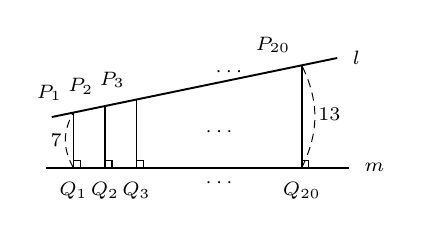
\begin{tikzpicture}[line width=0.6pt, x=0.50cm, y=0.50cm]
  \draw[line width=0.7pt] (0.3,0) -- (8.0,0) node[right=2pt, font=\scriptsize] {$m$};
  \draw[line width=0.7pt] (0.45,1.286) -- (7.70,2.786) node[right=2pt, font=\scriptsize] {$l$};
  \draw (1.0,0) -- (1.0,1.400);
  \draw (1.8,0) -- (1.8,1.566);
  \draw (2.6,0) -- (2.6,1.731);
  \draw (6.8,0) -- (6.8,2.600);
  \draw[line width=0.4pt] (1.0,0) -- (1.0,0.18) -- (1.18,0.18) -- (1.18,0);
  \draw[line width=0.4pt] (1.8,0) -- (1.8,0.18) -- (1.98,0.18) -- (1.98,0);
  \draw[line width=0.4pt] (2.6,0) -- (2.6,0.18) -- (2.78,0.18) -- (2.78,0);
  \draw[line width=0.4pt] (6.8,0) -- (6.8,0.18) -- (6.98,0.18) -- (6.98,0);
  \draw[densely dashed, line width=0.35pt] (1.0,0) to[bend left=30] (1.0,1.400);
  \draw[densely dashed, line width=0.35pt] (6.8,0) to[bend right=26] (6.8,2.600);
  \node[font=\scriptsize] at (0.56,0.70) {$7$};
  \node[font=\scriptsize] at (7.50,1.36) {$13$};
  \node[font=\scriptsize] at (4.70,0.90) {$\cdots$};
  \node[font=\scriptsize] at (4.95,2.42) {$\cdots$};
  \node[font=\scriptsize] at (4.70,-0.40) {$\cdots$};
  \node[font=\scriptsize, anchor=south east] at (0.96,1.44) {$\pt{P_1}$};
  \node[font=\scriptsize, anchor=south east] at (1.76,1.61) {$\pt{P_2}$};
  \node[font=\scriptsize, anchor=south east] at (2.56,1.77) {$\pt{P_3}$};
  \node[font=\scriptsize, anchor=south east] at (6.76,2.66) {$\pt{P_{20}}$};
  \node[font=\scriptsize, anchor=north] at (1.0,-0.12) {$\pt{Q_1}$};
  \node[font=\scriptsize, anchor=north] at (1.8,-0.12) {$\pt{Q_2}$};
  \node[font=\scriptsize, anchor=north] at (2.6,-0.12) {$\pt{Q_3}$};
  \node[font=\scriptsize, anchor=north] at (6.8,-0.12) {$\pt{Q_{20}}$};
\end{tikzpicture}
}\end{minipage}\par
\dmchoicesauto{}{$170$}{$175$}{$180$}{$185$}{$190$}
